\documentclass[10pt,a4paper,english]{book}
\usepackage{babel}
\usepackage{ae}
\usepackage{aeguill}
\usepackage{shortvrb}
\usepackage[latin1]{inputenc}
\usepackage{tabularx}
\usepackage{longtable}
\setlength{\extrarowheight}{2pt}
\usepackage{amsmath}
\usepackage{graphicx}
\usepackage{color}
\usepackage{multirow}
\usepackage{ifthen}
\usepackage[DIV12]{typearea}
% generated by Docutils <http://docutils.sourceforge.net/>
\newlength{\admonitionwidth}
\setlength{\admonitionwidth}{0.9\textwidth}
\newlength{\docinfowidth}
\setlength{\docinfowidth}{0.9\textwidth}
\newlength{\locallinewidth}
\newcommand{\optionlistlabel}[1]{\bf #1 \hfill}
\newenvironment{optionlist}[1]
{\begin{list}{}
  {\setlength{\labelwidth}{#1}
   \setlength{\rightmargin}{1cm}
   \setlength{\leftmargin}{\rightmargin}
   \addtolength{\leftmargin}{\labelwidth}
   \addtolength{\leftmargin}{\labelsep}
   \renewcommand{\makelabel}{\optionlistlabel}}
}{\end{list}}
\newlength{\lineblockindentation}
\setlength{\lineblockindentation}{2.5em}
\newenvironment{lineblock}[1]
{\begin{list}{}
  {\setlength{\partopsep}{\parskip}
   \addtolength{\partopsep}{\baselineskip}
   \topsep0pt\itemsep0.15\baselineskip\parsep0pt
   \leftmargin#1}
 \raggedright}
{\end{list}}
% begin: floats for footnotes tweaking.
\setlength{\floatsep}{0.5em}
\setlength{\textfloatsep}{\fill}
\addtolength{\textfloatsep}{3em}
\renewcommand{\textfraction}{0.5}
\renewcommand{\topfraction}{0.5}
\renewcommand{\bottomfraction}{0.5}
\setcounter{totalnumber}{50}
\setcounter{topnumber}{50}
\setcounter{bottomnumber}{50}
% end floats for footnotes
% some commands, that could be overwritten in the style file.
\newcommand{\rubric}[1]{\subsection*{~\hfill {\it #1} \hfill ~}}
\newcommand{\titlereference}[1]{\textsl{#1}}
% end of "some commands"
\ifthenelse{\isundefined{\hypersetup}}{
\usepackage[colorlinks=true,linkcolor=blue,urlcolor=blue]{hyperref}
}{}
\title{Developer guide}
\author{}
\date{}
\hypersetup{
pdftitle={Developer guide}
}
\raggedbottom
\begin{document}
\maketitle

\setlength{\locallinewidth}{\linewidth}
% comment: $Id: developer_guide.rst 128 2010-12-01 16:12:04Z s242720-studenti $ 
% comment: the order for section decorations is : _ . ' ` 
\begin{center}\begin{sffamily}
\fbox{\parbox{\admonitionwidth}{
\textbf{\large Hint}
\vspace{2mm}

Welcome to the developer guide for the SVG whiteboard. The
table of contents may seem huge, but many sections are really
short. You can always click on section titles to come back to the
contents table.

A short description of the contents and why to read them:
\begin{itemize}
\item {} 
Code structure: read this to understand the general structure
behind the current code and get a first orientation

\item {} 
Data structure: refer to this section (especially the \href{\#whiteboard-database}{\ref*{whiteboard-database}} section) to understand the structure of variables that
are accessed and modified. This section is useful as a reference
even after you are confident with the code structure.

\item {} 
Specific solutions: a place for reminders for taken project
choiches and technology findings

\end{itemize}
}}
\end{sffamily}
\end{center}
\hypertarget{contents}{}
\renewcommand{\contentsname}{Contents}
\tableofcontents

\bigskip
\label{contents}


%___________________________________________________________________________

\hypertarget{main-principle}{}
\chapter{Main principle}
\label{main-principle}

The leading idea behind the application is a lightweight interaction
model which, combined with the capabilities of vector graphics, allows
to support a shared whiteboard through the exchange of few textual
messages.

The textual representation of vector graphics is common knowledge, and
is easy to understand how this can enable to transmit graphic data
with short communication messages (although in some cases this
advantage may fail). I will focus now on the overall sharing model,
thought to provide each client with an updated state of the
whiteboard.

The fundamental event that triggers the evolution of the application,
is an user \textbf{action}, that is a change on the user whiteboard that is
supposed to be propagated to all other clients. To mantain an updated
state, the actions get propagated one by one when executed, even if
some of them could nullify the effect of some others (like for a
deletion of a created object).

Each \textbf{action} is represented by a textual \textbf{update} which contains
all relevant informations about what the user did. The main purpose of
the server side of the application is to manage the distribution of
these updates.

The web technology prevents the client side code to directly
communicate with other clients, so an extern server is
compulsory. Moreover, the same technology prevents the clients to
directly receive updates in a \emph{push} manner (websockets in html5 are
going to provide push methods to client in the future), so a server is
needed to provide updates in response of \emph{pull} requests (see
\href{\#emulating-a-client-push-behavior-with-the-http-technology}{\ref*{emulating-a-client-push-behavior-with-the-http-technology}} for
performance details).

So the server role is to manage an \textbf{update database} so that each
client can ask for new updates, depending on his own state. With the
access to a writable storage device, that is very common even on the
smallest web servers, the server can manage a bigger update database,
and mantain all the state of a whiteboard, since its creation, in this
action-oriented form.

The following image illustrates a simple case of update
management. Here you can immediately see some important elements that
constitute the application's internals:
\begin{itemize}
\item {} 
The \textbf{update database}, that is the main data structure on the
server

\item {} 
The two principal requests made from the clients to the server, that
are the \textbf{read} and the \textbf{write} requests

\end{itemize}

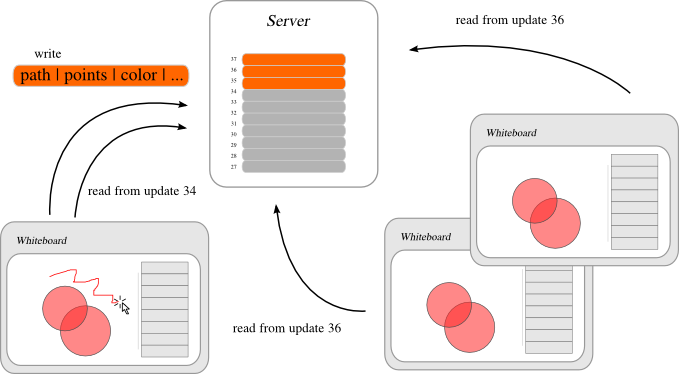
\includegraphics{images/base_principle.png}

The update is sent, usually, when the user terminates an operation, be
that a move, create or edit action. Then the update is sent to the
server (this is a request with the \texttt{mode} parameter set to
\texttt{write}), which gives it a numerical incremental identificator and
adds it to the database. At the same time, several clients are asking
for updates sending a request with \texttt{mode} set to \texttt{read}, including
the identificator of the next update which they are interested in.


%___________________________________________________________________________

\hypertarget{elements-involved}{}
\section{Elements involved}
\label{elements-involved}

In this case, the main parts of the software which are running are:
\begin{itemize}
\item {} 
for the addition of a new update, the global \textbf{sender} object
(\texttt{g{[}'sender'{]}}) on the client side and the \texttt{write} \textbf{mode} on the
server side

\item {} 
for the request about new updates, the global \textbf{receiver} object
(\texttt{g{[}'receiver'{]}}) on the client side and the \texttt{read} \textbf{mode} on the
server side

\end{itemize}


%___________________________________________________________________________

\hypertarget{server-mode-parameter}{}
\section{Server \texttt{mode} parameter}
\label{server-mode-parameter}

I mentioned above the server's \texttt{mode} parameter, this is the main
query field determining the kind of the server's response.

The server side code is structured following a functional programming
paradigm, on the purpose of making the execution flow as clear as
possible. We have the two certain boundaries of this flow, that are
the start by a user request, and the end by a response to the user, so
the different server behaviors are conceived like parallel ways on the
same path, in a few words they are the branches of a big \texttt{switch}
control structure, and the \texttt{mode} parameter is the one that
determines which way will be taken. Take a look at the \texttt{main.php}
file to easily verify what explained.


%___________________________________________________________________________

\hypertarget{principal-division-of-the-application}{}
\section{Principal division of the application}
\label{principal-division-of-the-application}

The main elements constituting the application's structure are:
\begin{itemize}
\item {} 
Client side code (\texttt{client/} directory)

\item {} 
Server side code (\texttt{server/} directory)

\item {} 
Stored data (\texttt{data/} directory)

\end{itemize}

All of them reside on the webserver, in a form optimized by the
makefile, but their original structure is intended to help a developer
to move through the code and clearly understand what is being done.  I
will write here about the server side and client side code, while for
the form of the stored data see the section \href{\#stored-data}{\ref*{stored-data}} under \href{\#data-structures}{\ref*{data-structures}}.

The client and server side of the source code are documented into the
following section, \href{\#code-structure}{\ref*{code-structure}}, while the data are documented
into \href{\#data-structures}{\ref*{data-structures}}, together with the meaning of complex
variables used into the code.


%___________________________________________________________________________

\hypertarget{code-structure}{}
\chapter{Code structure}
\label{code-structure}

In this section I will present the main structures thought to organize
the code. The order of the subsections reflects the importance of each
topic. The first two subsections deal with those structures limited to
the client or the server side, while the following sections present
topics which involve both sides of the application.


%___________________________________________________________________________

\hypertarget{client-side}{}
\section{Client side}
\label{client-side}

Following a general rule of network protocols, I've tried to move the
biggest part of the computational load towards the network boundaries,
that means towards clients, leaving it off from the server.

Current hardware performances for an average web browser aren't an
heavy limit for this kind (strongly interactive) of applications, or
at least I couldn't observe any performance problem related to
javascript on the testing machine (and virtual machine), which runs on
quite old hardware (see \href{\#hardware}{\ref*{hardware}}).

The biggest problem I met was therefore that of readability and
decomposition of the client side code.

The starting code was all based on global variables, and I choosed to
proceed by steps, instead of trowing away the existing structure. The
resulting code has an hybrid programming paradigm, being object
oriented just in some of his parts\footnotemark[1].

The javascript code is divided among files in a way that follows the
graphical division of the user interface, as shown in the image below:

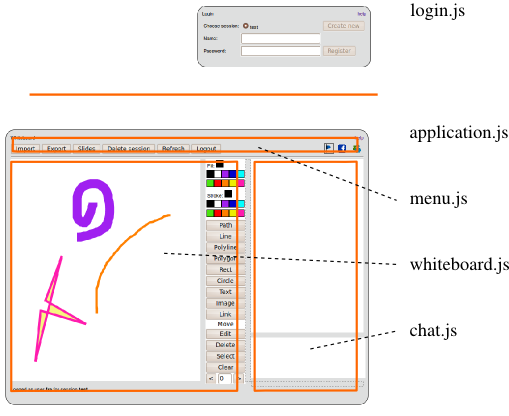
\includegraphics{images/client_surface.png}

The javascript function definitions can be found on the file
corresponding to the zone of the page containing the html element to
which the method is associated. For example, this html code can be
read about the ``Import'' button, which is contained into the menu:
\begin{quote}\begin{verbatim}
<button onclick="show_div('menu_import', true)">Import</button>
\end{verbatim}
\end{quote}

Since the ``Import'' button is contained into the menu, the programmer
will find the \texttt{show{\_}div} function declaration inside menu.js.

Another consequence of the shown division is that there are two
javascript files, \texttt{login.js} and \texttt{application.js}, which are
associated to a whole html page. Thus the initialization functions for
each page are contained into the corresponding file; see the next
section for details about the one contained in \texttt{whiteboard.js},
which is the more complex.

To be complete, it's better to immediately consider another image
which introduces also those javascript files not directly associated
to a visible surface of the user interface. The image illustrate the
use relationships between the javascript files, a very useful
information while browsing the code:

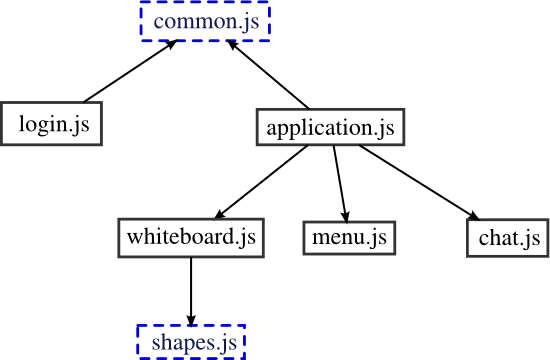
\includegraphics{images/client_file_use.png}

An arrow from a start file to an end file means that the code of the
start file calls some functions which are defined into the end
file. Two new informations come from the structure of the diagram:
\begin{itemize}
\item {} 
the role of \texttt{common.js} that is like a little shared library for
common tasks (the most important thing, it contains the channel
class)

\item {} 
the presence of the \texttt{shapes.js} file (containing the shape class
and all shape objects derived from that), which is used exclusively
by functions into \texttt{whiteboard.js}

\end{itemize}

The introduced division of client side code it not totally rigid,
there are still dependencies, here and there, between variables
defined into different files. I've tried to collect into common.js the
variables, functions and objects used by several files, like the
global object \texttt{g} holding all global variables, and the \texttt{channel}
and \texttt{signer} objects.


%___________________________________________________________________________

\hypertarget{dispatching-the-execution-flow-through-the-files}{}
\subsection{Dispatching the execution flow through the files}
\label{dispatching-the-execution-flow-through-the-files}

On the purpose of decomposing the client logic, also global variables
are defined within the files where they are used. When the client side
state is initialized, several functions are called, each one to
initialize the variables belonging to a file.

The main initialization function is defined into \texttt{application.js};
it initializes the variables defined into \texttt{application.js} and than
calls the initialization functions for the file \texttt{whiteboard.js} and
\texttt{menu.js}:
\begin{quote}\begin{verbatim}
window.onsvgload = function() {
    ...
    initWhiteboard();
    initMenu();
    ...
};
\end{verbatim}
\end{quote}

A similar approach is used when an update is received by the
client. The \texttt{receiver{\_}handler} function (into \texttt{application.js})
calls the specific functions belonging the the files \texttt{whiteboard.js}
and \texttt{chat.js}, since within those files the developer will found all
functions needed to process the update of the right type:
\begin{quote}\begin{verbatim}
function receiver_handler(){
    ...
    if (action == 'chat')
        chatServerUpdate(madeBy, objId, parameters, time);
    else{
        ...
        whiteboardServerUpdate(objId, page, action, parameters);
        }
    ...
}
\end{verbatim}
\end{quote}

Note that the approach used for the initialization and for the
processing of an update is a total waste of resources, from the
computational point of wiew. It is just an effort to organize the code
for the developer.


%___________________________________________________________________________

\hypertarget{object-implementation-on-the-client-side}{}
\subsection{Object implementation on the client side}
\label{object-implementation-on-the-client-side}

The javascript language is very flexible when it comes to object or
class definition, due to his prototypal model and the possibility of
dynamically add member functions and internal variables to the
objects. Although an uniform programming style is important for
readability and to avoid mistakes, the few javascript objects are
defined in different ways, depending on their lifecycle.

All the objects that will be created dynamically (\texttt{line}, \texttt{circle}
and all the shapes, and the \texttt{shape} and \texttt{channel} classes) are
defined through their constructors, while permanent singleton objects
(\texttt{g{[}'signer'{]}}, \texttt{g{[}'sender'{]}}, \texttt{g{[}'receiver'{]}}, \texttt{g{[}'pages'{]}}
and \texttt{g{[}'size{\_}adapter'{]}}) are directly built and assigned to the
global variable where they will remain.


%___________________________________________________________________________

\hypertarget{the-channel-class}{}
\subsection{The channel class}
\label{the-channel-class}

The channel class provides an ajax channel to the server, with some
functions to send the request, handle errors, and retry the request
after a timeout. A channel object is contained (and used) by all other
objects which need to exchange data with the server in an asynchronous
manner.

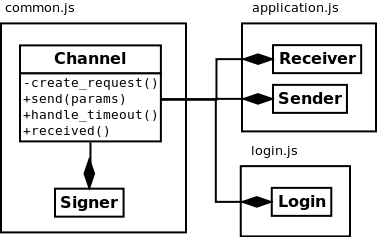
\includegraphics{images/Channel_use_diagram.png}

The responsabilities of the channel class are:
\begin{quote}
\begin{itemize}
\item {} 
Create, send and receive an ajax request in a way which is
supported cross-browser

\item {} 
Handle the case of timeout of the sent request, sending again the
same request

\end{itemize}
\end{quote}

These functions are used by the \texttt{login} and \texttt{sender} objects to
send individual messages, and by the \texttt{receiver} and \texttt{signer}
objects to send messages in a cycle.

The structure of objects using \texttt{channel} is a little messy, because
the channel object needs methods which are exposed on the global
scope, in order to assign them as handlers for timeout and ajax
statechange events. For example, the \texttt{g{[}'sender'{]}} object defines
two global methods that are assigned to the channel object during its
initialization (code taken from \texttt{application.js}):
\begin{quote}\begin{verbatim}
// Sender initialization
g['sender'].channel =
    createChannel(sender_handler, sender_timeout, 10000, send_par);

// Sender object and methods
g['sender'] = {
    ...
};
function sender_timeout(){
    g['sender'].channel.handle_timeout();
}
function sender_handler(){
    ...
}
\end{verbatim}
\end{quote}

The methods must be defined outside of the object, which is not very
elegant, but it is the only way. Moreover, you can observe that the
\texttt{sender{\_}timeout} method just calls a method into the channel
object. This is even less elegant and this is done by all objects that
use a channel object, because it is difficult in javascript to assign
an inner method of an object as handler for an event like the timeout.


%___________________________________________________________________________

\hypertarget{client-send-buffer-and-the-sender-object}{}
\subsubsection{Client send buffer and the \texttt{sender} object}
\label{client-send-buffer-and-the-sender-object}

The channel class is used by two important objects, the \emph{sender} and
the \emph{receiver}; both of them are defined into the file
\texttt{application.js}. The channel class itself handles the failure and
resend of ajax requests, but the sender object needs anyway a buffer
to temporarily store the updates produced by the user.

The function that adds a new update to the buffer (server{\_}add) has the
following interface:
\begin{quote}\begin{verbatim}
sender_add(action, parameters, varidObj, async)
\end{verbatim}
\end{quote}

All parameters but \texttt{action} are optional, and the last (\texttt{asinc})
is useful to add a new update line into the database without trying to
flush it. Indeed, \texttt{sender{\_}add} usually tries to flush the buffer
right after it's execution, but when the user edits a shape, for
example, it is better if the old shape's deletion and the new shape's
creation are sent to the server at the same time.

The sender channel (like all other objects that use the \texttt{channel}
class) waits that an old ajax request has succeeded before sending a
new one. When the \texttt{sender} object receives a response from the
server, it checks its buffer for updates collected in the meantime
since the request was sent.

Here it is the relative code (into application.js). The response
handler (sender{\_}handler) can call again the send function (line 7):
\begin{quote}\begin{verbatim}
1  function sender_handler(){
2      var response = g['sender'].channel.received();
3      if(response !== false){
4          // If still have data to send (added while waiting the server
5          // response)
6          if (g['sender'].line_buff.length > 0)
7              sender_send();
8      }
9  }
\end{verbatim}
\end{quote}

For all objects which use the \texttt{channel} class, the handling of a
failure (a \texttt{false} response received by the channel class) is a
delicate matter. A \texttt{false} response is returned every time that, for
example, the readyState of the response is not the right one, so the
handler receiving from \texttt{channel} should simply ignore the call and
do nothing. This interface, however, is likely to be changed because
explicit errors (see next section) are better handled by the specific
handler receiving from channel.


%___________________________________________________________________________

\hypertarget{handling-of-ajax-errors}{}
\subsubsection{Handling of AJAX errors}
\label{handling-of-ajax-errors}

The \texttt{channel.received} method is called by \texttt{channel} users each
time that the XMLHttpResponse object changes its state, and the
\texttt{ready} state is only the forth, so many times the method simply
returns the \texttt{false} value to tell to its caller that the moment
isn't already arrived.

Besides receiving a correct ready response, several kind of errors can
occurr while the \emph{channel} class is awaiting. First I will present the
different kind of errors, and then I will tell how they are handled.
\begin{itemize}
\item {} 
\textbf{malformed XML} This can cover a variety of errors: during the development these are
usually php errors which output the details of the error instead of
the XML response. Sometimes, with explorer (6), these errors can be due
to a malformed ajax request, which occurs randomly and which is not
repeated by the browser if the request is resent.

A problem in the handling of this errors is that there isn't a
method to verify the valid XML structure of the response (into the
class XMLDocument), so an exception could be risen when upstream
code tries to parse the received response. Thus to try to locate XML
errors, I try to access to the last nodes or to the whole first
level of child node, but this method is not sure, it depends from
the parser implementation:
\begin{quote}\begin{verbatim}
try{
    var response = this.request.responseXML.documentElement;
    // These are used to force explorer (and other
    // browsers) to parse the XML document to spot errors
    response.lastChild;
    response.childNodes;
}
catch(e){
    // *malformed response*: this could even be a php
    // error. Firefox raises an exception on
    // this.request.responseXML while Explorer should raise an
    // exception on response.lastChild
    var msg = 'A server error occurred:\n\n'+this.request.responseText;
}
\end{verbatim}
\end{quote}

\item {} 
\textbf{Http errors} They are signaled to the client side code with a request whose state
is 'ready' but whose 'status' is different from 200. This includes
the case of an unreachable server (http status '0').

\item {} 
\textbf{Timeouts} When the response doesn't comes within the timeout.

\item {} 
\textbf{Explicit errors} These are errors sent on purpose by the server
to the client, in order to show an error message client-side or to
impose a behavior (for example: logout). This is told to the client
through an \texttt{error} XML tag.

\end{itemize}

About the handling of these errors, the first distinction is about the
\textbf{explicit errors}: they are different within different channels, so
they are handled outside of the channel. Other kind of errors may
occur with all channels and are handled within the
\texttt{channel.received} method.

A \textbf{malformed XML} response or an \textbf{http error} are handled the same
way: a message is prompted to the user, trying to be as clear as
possible, and he can decide if to repeat the request or to give up (in
this case he will be logged out from the whiteboard). This behavior
works well with the case of a server complaining for a malformed ajax
request, which occurs randomly with explorer (this triggers a
malformed XML error). This works well also when an http error is given
due to a server not responding (the user may notice, for example, that
his network is down and retry).

A \textbf{timeout} error simply triggers a new send with the same
parameters, and the user is warned with a subtle notification but he
doesn't has to decide anything.


%___________________________________________________________________________

\hypertarget{the-deletion-of-a-whiteboard-on-the-client-side}{}
\subsubsection{The deletion of a whiteboard on the client side}
\label{the-deletion-of-a-whiteboard-on-the-client-side}

The deletion of a whiteboard while several users are working on it is
an event which can lead to the failure of several server side
operations. Simultaneusly, several ajax requests made from the client
side may fail, and I decided to not take care of each one of these
failures, but to rely on the failure of the whiteboard's heartbeat:
the 'receive cycle'.

The whiteboard is almost\footnotemark[6] always awaiting for a response from
the server, because of the \texttt{g{[}'receiver'{]}} object and the receive
cycle it manages, so I demanded to this object the handling of the
\texttt{whiteboard deleted} \textbf{explicit error} (see section above), which
leads to the logout of the user from the whiteboard. Other client-side
failures due to a deleted whiteboard are simply ignored, relying on a
prompt reaction of the receiver object.


%___________________________________________________________________________

\hypertarget{the-shape-class}{}
\subsection{The shape class}
\label{the-shape-class}

The \textbf{shape} class came from the attempt to simplify the code running
into the whiteboard. This class is used only through its derived
classes (it can be seen as an abstract class) and by the functions
into the file \texttt{whiteboard.js}.

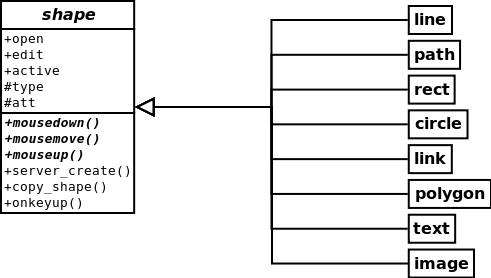
\includegraphics{images/Shape_derivation_diagram.png}

This diagram shows only the public methods, for the protected ones see
the next figure. The shape class has mainly three virtual methods
(mousedown, mousemove, mouseup), which must be overridden by the
derived shapes, even if the language syntax doesn't provides any
keywork to indicate virtual methods.

The idea behind this class is that when an user chooses a tool that
corresponds to a shape, all mouse (and keyboard) actions inside the
canvas get forwarded to the corresponding shape class, and the class
decides how to handle the mousedown, mousemove, and mouseup
events. This structure aims to achieve both modularity and flexibility
in the definition of classes.

There are two kind of shapes derived from \texttt{shape}:
\begin{itemize}
\item {} 
\textbf{dynamic shapes}: they are the most part. In this case a shape
corresponds tightly with an SVG element, and many methods can
automatically copy attribute values from the shape to the server or
to the SVG element. The aspect of these shapes changes while the
user is creating them, but they are created all together on the
canvas of the other users receiving the update.

\item {} 
\textbf{static shapes}: these are the \textbf{text}, \textbf{link}, and \textbf{image}
shapes. They are created within a single function, because the
intermediate state is constituted by a text that the user changes
into the textarea. For these shapes, the correspondence with an SVG
element is less tight, because their actual structure on the svg
canvas is more complex; this is the reason why all static shapes
override the \texttt{server{\_}create} method.

\end{itemize}

This distinction doesn't corresponds with any structure into the code,
but it helps to understand the different use of \texttt{shape} protected
methods on part of his derived shapes. These protected methods are the
part of the base class which can be used by several shapes with a
similar behavior.

\texttt{shape} protected methods are defined on two levels, a first level
of methods which is used by the second level. Usually, derived shapes
use the second level, but sometimes they can need customization and
rise up to the first level (this is the case of the \emph{path} shape,
which needs to build custom groups to handle the creation of
multipaths). This simple diagram shortly describes the relationships
between the protected methods into the shape class:

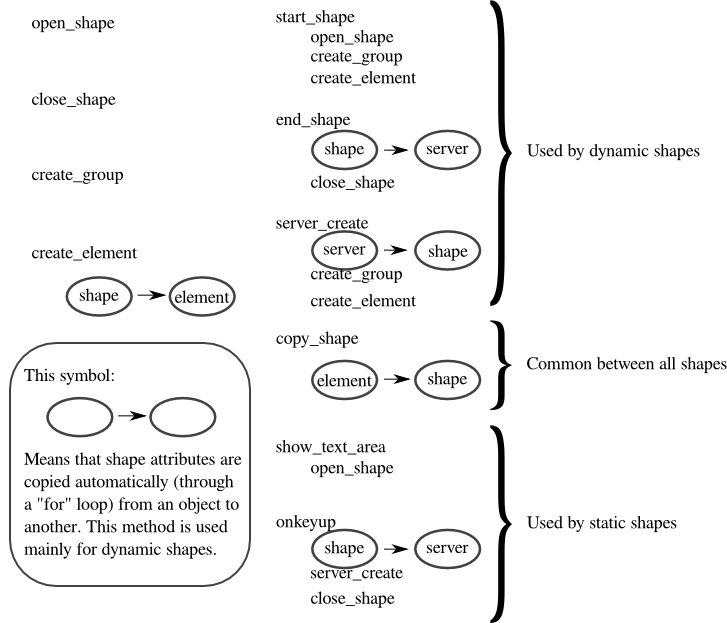
\includegraphics{images/shape_protected_methods.png}

The methods on the first column can be thought as a first level, and
the ones on the second column as a second level. These are not all
protected methods (some are public), but they are all methods which
are reused inside the derived shapes.

The meaning of the words into the ellipses is:
\begin{itemize}
\item {} 
shape: the shape object (has attributes as object properties)

\item {} 
element: the SVG element (his attributes correspond to visual properties)

\item {} 
server: the server update (attributes are encoded as an ordered array)

\end{itemize}

This skecth can be useful to get an idea of the overall structure, but
many details are missing which can be found in the code.


%___________________________________________________________________________

\hypertarget{random-remarks-on-the-structure-of-the-shape-class}{}
\subsubsection{Random remarks on the structure of the shape class}
\label{random-remarks-on-the-structure-of-the-shape-class}

The methods \texttt{open{\_}shape()} and \texttt{close{\_}shape()} handle the \texttt{open}
flag; this is read upstream to know if the shape is open (an user
can't change his tool if he has an unclosed shape).

The method \texttt{copy{\_}shape} sets also the \texttt{edit} flag true. All
derived shapes can change their behavior when the shape is in edit
mode.

Usually a shape remains alive during all the time while the
corresponding tool is selected, continuously generating new elements
and server updates. On the other hand, with the edit tool a shape is
copied by an existing one, and it shouldn't generate new shapes after
that the editing is finished. For this reason, when an edited shape is
closed, its \texttt{active} flag is set to false, so that the upstream code
can understand that no more shapes of that type should be created
(\texttt{close{\_}shape} method).


%___________________________________________________________________________

\hypertarget{client-side-concurrency}{}
\subsection{Client side concurrency}
\label{client-side-concurrency}

Even if I couldn't find a clear specification of the behavior of the
javascript language with respect to concurrency, from several articles
found on the web and from the practice it results that javascript
doesn't supports preemption, thus an event is handled after that the
current block has ended.

To avoid concurrency problems, is thus necessary to mantain the
coherence of global variables within each function that changes
them. This is easier for the new parts of the code which are
structured following the object oriented paradigm.

Sometimes (\texttt{sender{\_}handler} function inside \texttt{application.js},
\texttt{login{\_}handler} function inside \texttt{login.js}) when receiving an ajax
response from the server, the underlying datas are checked, to be sure
that the response is still valid or to know if a new request should be
sent.


%___________________________________________________________________________

\hypertarget{server-side}{}
\section{Server side}
\label{server-side}

The server side is decomposed following a procedural paradigm, which I
think is better to describe the control flow in this case. However, to
reduce the complexity of function interfaces, some of their parameters
have been packed into an associative array (see \href{\#the-client-identifier}{\ref*{the-client-identifier}}).

The choice of a procedural decomposition came from the consideration
that the server code doesn't actually follows complex control flows,
but instead the whole logic is started with each user request and ends
with a response to that user, changing eventually the database as an
important side effect.


%___________________________________________________________________________

\hypertarget{the-main-switch}{}
\subsection{The main switch}
\label{the-main-switch}

The execution flow is described in its principal steps into the
\texttt{main()} function, where I tried to balance the readability (that
means hiding the code by incapsulation) with the expression of the
underlying logic.

To achieve this goal, there is a separation of functions into groups,
and the structures into \texttt{main()} do the association between the user
request and the corresponding functions.


%___________________________________________________________________________

\hypertarget{function-groups-and-server-side-files}{}
\subsection{Function groups and server side files}
\label{function-groups-and-server-side-files}

The function used by \texttt{main()} are mainly grouped into two types:
\begin{quote}
\begin{itemize}
\item {} 
modifying the database (file \texttt{updates.php}): The functions that
modify the database are all defined into \texttt{udpates.php}, so that
the database structure is somehow encapsulated into this file. The
file contains the functions called by \texttt{main()}, but it contains
also functions called just internally, and defined to reuse the
code or to improve the readability

\item {} 
formatting the output (file \texttt{markup{\_}send.php}): Here, all the
functions that write HTML or XML are defined, to wrap the data
received upstream by \texttt{main()}, and to send them to the user.

\end{itemize}
\end{quote}

Sometimes, this division turns into an excessive rigidity, and
sometimes (in the case of \texttt{export{\_}chat}) a function into updates.php
also cares for formatting, but this remains a guideline into the
structure of the server side code.

With the grouping of functions into the files and the procedural
decomposition model I used, it is easy to follow the execution flow
through the various files that compose the server side code. The
following diagram shows the use relations between server side files
(the \texttt{.php} extension is omitted) when an user sends a request. An
arrow starting from a file and arriving into another file means that
the first file is using a function from the second one.

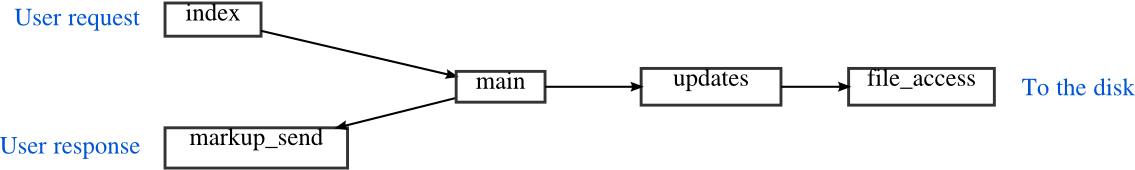
\includegraphics{images/server_file_use_simplified.png}

As can be seen, from the \texttt{main} file the execution flow goes to the
\texttt{update} functions, which in turn call the functions from
\texttt{file{\_}access} to read and write the update database copy on the
disk. When the \texttt{update} functions give back the control flow to the
\texttt{main} file, it uses the returned values to call the functions into
\texttt{markup{\_}send}, to send back the response to the user.


%___________________________________________________________________________

\hypertarget{steps-for-the-server-response}{}
\subsection{Steps for the server response}
\label{steps-for-the-server-response}

The presented function groups correspond also with two steps of the
server operation, and so they can be found used into two successive
switches inside \texttt{main()}: a firs one based on the \texttt{mode} parameter
that chooses among which \emph{update} function to use, and a second one
based on the \texttt{{\$}o{[}'type'{]}} (output type) parameter that chooses among
which \emph{markup send} function to use\footnotemark[2].

The \emph{markup send} step is born to collect formatting functions that
were common between several \emph{modes}, so the output functions for the
\texttt{export} mode remain outside from this step: they stay into the
\texttt{export} branch of the \emph{update} switch, since they are used just
there. The \texttt{export} mode is quite different from the others, and the
\href{\#export-mode-and-draw-image}{\ref*{export-mode-and-draw-image}} section covers its characteristics.


%___________________________________________________________________________

\hypertarget{the-client-identifier}{}
\subsection{The client identifier}
\label{the-client-identifier}

The drawback of a procedural decomposition paradigm is that many
functions belonging to the same processing step could require the same
data set, resulting in big and redundant function interfaces. For
example, the functions belonging to the \emph{update} step often need
informations about the user which sent the request, his user id (to
improve performances reducing database search), and the name of the
whiteboard where he is operating.

I packed all these variables into the variable \texttt{{\$}client{\_}id}, which
is a parameter of all the functions of the \emph{update} step. The variable
is sent by the client or produced by the \texttt{login} function in the
form of a joined array with the structure:
\begin{quote}\begin{verbatim}
<user id> . '_' . <user name> . '_' . <whiteboard name>
\end{verbatim}
\end{quote}

And it is parsed by \texttt{parse{\_}client{\_}id} into an associative array, to
provide textual keys to the functions. This array can be found as a
parameter of almost all \emph{update} functions.


%___________________________________________________________________________

\hypertarget{export-mode-and-draw-image}{}
\subsection{Export mode and draw{\_}image}
\label{export-mode-and-draw-image}

This mode deserves a specific coverage, because is more complex than
all the other methods and requires a whole file (\texttt{draw{\_}image.php})
just to accomplish the operations required to export the whiteboard
contents.

The complexity arises from two factors:
\begin{description}
\item[{Database structure}] \leavevmode 
The server doesn't actually sees the current state of the
whiteboard, but it simply keeps the received updates. Thus, only
for this mode, it must walk through the whole database and
transform the update list into a structure reflecting the status
(the \texttt{{\$}objects} variable). This task has been incapsulated into
the \texttt{export{\_}whiteboard} function (\texttt{updates.php}).

\item[{Format encoding}] \leavevmode 
A change from one format to another, which is simple a matter of
changing a form value for the user, entails whole sets of
different operations into the server side code, since the functions
may change for each object type. This task has been incapsulated
into the \texttt{draw{\_}image} function (\texttt{draw{\_}image.php}).

\end{description}

The \texttt{export{\_}whiteboard} function does also all operations which will
be useful for every kind of export format, for example it parses
complex action parameters and it translates the sizes from global
units to local units (see \href{\#global-and-local-measure-units}{\ref*{global-and-local-measure-units}}); this
makes the two tasks (the production of the \texttt{{\$}objects} variable and
its output as a file for the user) tightly coupled but the division
between them seems reasonable to me to organize the code.

All the code for the export mode is strongly dependent by the position
of the parameters into each update string. This is a problem for
readability and maintainability, that I discuss into \href{\#joined-arrays-for-the-action-parameters}{\ref*{joined-arrays-for-the-action-parameters}}, where I introduce some ideas to change the
current structure.

Now that this mode has been presented, I can show the full use diagram
between server side files, including even those files which are
secondary and related to this specific mode:

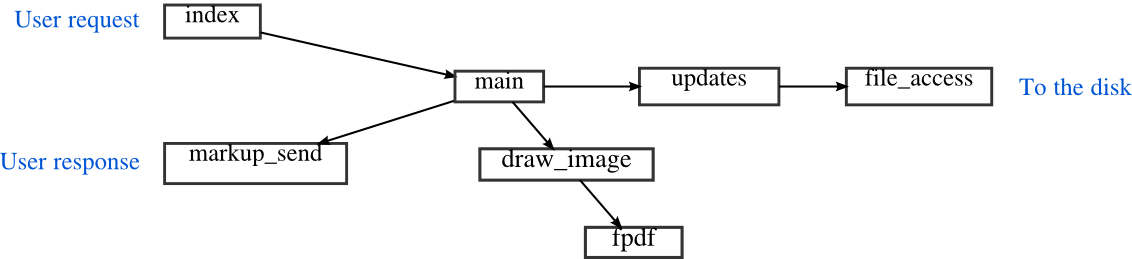
\includegraphics{images/server_file_use_full.png}


%___________________________________________________________________________

\hypertarget{server-side-concurrency}{}
\subsection{Server side concurrency}
\label{server-side-concurrency}

On the server side, concurrency problems arise for the access to the
shared files on the disk (see \href{\#stored-data}{\ref*{stored-data}} for an overview of such
files). As seen into the section \href{\#function-groups-and-server-side-files}{\ref*{function-groups-and-server-side-files}}, all the functions that read and write disk files are grouped
together into the file \texttt{file{\_}access.php}, so these are the functions
which also handle the problem of concurrency\footnotemark[3]. All
these functions are called just by other functions defined in
\texttt{updates.php}, with the exception of \texttt{check{\_}files()}.

First of all, some of the files do not present concurrency problems:
the \emph{permissions} file is read-only (writable only by hand by the
administrator) and the \emph{log} file is write-only.

The changing and shared files are:
\begin{quote}
\begin{itemize}
\item {} 
the \textbf{passwords} file

\item {} 
the \textbf{whiteboard} database for each whiteboard

\item {} 
the image folder for each whiteboard

\end{itemize}
\end{quote}

The passwords file and the whiteboard databases may change
their content, while both the whiteboard databases and the image
folders may exist or not exist at all.


%___________________________________________________________________________

\hypertarget{encoded-files}{}
\subsubsection{Encoded files}
\label{encoded-files}

The \textbf{passwords} file and the \textbf{whiteboard} database files have the
common property of being an encoded form of a php array. The functions
accessing to these files (whiteboard{\_}create, whiteboard{\_}delete,
file{\_}create, \textbf{file{\_}get} and \textbf{file{\_}put}) handle both the variable
encoding/decoding and the concurrent access.


%___________________________________________________________________________

\hypertarget{use-of-file-get-and-put}{}
\subsubsection{Use of file get and put}
\label{use-of-file-get-and-put}

Both the definition and the use of \texttt{file{\_}get} and \texttt{file{\_}put} are
straightforward\footnotemark[4]. Into the file \texttt{updates.php}, all
actions executed between a \emph{write file{\_}get} and a file{\_}put can be
thought as acting on an exclusive locked version of the database. I
wrote \emph{write file{\_}get} because this function can be called with a read
(\texttt{r}) or a read write (\texttt{rw}) value as mode argument; when it is
called with a \texttt{rw} mode, it returns also an handler, which must be
given back to file{\_}put to terminate the critical section.
\begin{quote}\begin{verbatim}
list($h, $d) = file_get($wb_file, 'rw');
...
file_put($h, $d);
\end{verbatim}
\end{quote}

The second parameter of \texttt{file{\_}put} is useful to tell to the function
that the data have been modified, and so they must be written on the
file. Sometimes, functions into \texttt{updates.php} can open the file with
the \texttt{'rw'} mode but don't actually modify the data, in this case
they can use \texttt{file{\_}put({\$}h)} simply omitting the second parameter.


%___________________________________________________________________________

\hypertarget{double-locking-level}{}
\subsubsection{Double locking level}
\label{double-locking-level}

Each \textbf{whiteboard} database file can be accessed independently, so
the locking should be done singularly over each of those
files. However, since those files can be existent or not, a prior
atomical check must be done on file existence, so the locking of
whiteboard database files has two levels. Since the \textbf{passwords} file
is accessed through the same functions, the double lock is used also
for that file, even if this is not strictly necessary.

The files mentioned above are accessed through the following four
functions, which use a global lock file and a local lock file for each
operation:
\begin{itemize}
\item {} 
whiteboard{\_}create, whiteboard{\_}delete, file{\_}create (for passwords file)

\item {} 
file{\_}get, file{\_}put

\end{itemize}

The following image represents the use of lock files with symbols, to
easily check that they are used properly. The global lock (the red
one) is used to protect file creation and deletion, that is changes to
the filesystem, while the local lock is used for changes within a
specific whiteboard database or folder.

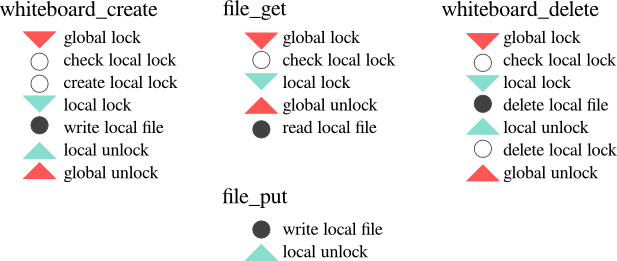
\includegraphics{images/server_concurrency.png}

The existence of different local locks is very important when users
are working on different whiteboards on the same server.

With this model, a file{\_}delete can remain blocked on the local lock if
a file get/put has to finish, but it happens rarely that a whiteboard
is deleted so this is not a problem for performances.


%___________________________________________________________________________

\hypertarget{whiteboard-existence-and-automatic-logout}{}
\subsubsection{Whiteboard existence and automatic logout}
\label{whiteboard-existence-and-automatic-logout}

All functions into \texttt{updates.php} which read the whiteboard database
are subject to failure if the whiteboard has been deleted. Usually
when a whiteboard is deleted the first function which fails is the
\texttt{read} function which is waiting in a long polling cycle.

When the \texttt{read} function fails, an explicit error message is sent to
the client functions which handle the XML response, and those
functions force the user to log out.

This is the reason why it is very difficult that another function can
fail for an unexistent whiteboard, because usually users are forced to
log out as soon as the whiteboard is deleted. This is the reason
because error handling is not very important for a missing whiteboard,
for all functions but the \texttt{read} function.


%___________________________________________________________________________

\hypertarget{permission-file-access}{}
\subsubsection{Permission file access}
\label{permission-file-access}

This file is accessed just through the function \texttt{check{\_}permissions},
and if the file doesn't exist the function creates on its first
invocation. The concurrent access on this file can in the worst case
create it two times with the same default content, while for the rest
of the application life the file is accessed just for reading.


%___________________________________________________________________________

\hypertarget{emulating-a-client-push-behavior-with-the-http-technology}{}
\section{Emulating a client \emph{push} behavior with the http technology}
\label{emulating-a-client-push-behavior-with-the-http-technology}

When using a pull update technique, there is a trade-off on the
frequency of client update requests. Frequent requests improve the
responsiveness to changes made from other users, but increase the
network load, and the server and client overhead (although the latter
is negligible).

In this application, a behavior similar to a pull-like one is achieved
simply delaying the response send to the client that asked for
updates. If an updates request comes to the server while no new
updates are available, the response is delayed by a configurable
amount of time during which the server process periodically checks the
presence of new updates, until a new one is found or the number of
retries becomes too high. After a given number of retries with no new
updates, the server replies to the client with an empty response.

The cost of this technique is that of a suspended server process for
each client, that periodically wakes up and opens the database for
reading.

Here it is a simplified snippet of code taken from the server side
function 'read', which handles the response to a client update
request. At lines 2 and 4, \texttt{{\$}server{\_}update{\_}retry} and
\texttt{{\$}server{\_}update{\_}timeout} are two parameters configurable into the
file \texttt{configuration.php}.
\begin{quote}\begin{verbatim}
 1    // The time interval between each check
 2    $update_wait = (int)$server_update_timeout/$server_update_retry;
 3    // wait until we find new ids, or until maximum retry number
 4    for ($i = 0; $i < $server_update_retry; $i++) {
 5        // Read the database and retrieve the latest id
 6        $d = file_get($c['wb_file'], 'r');
 7        if ($d['next_upd_id'] > $id)
 8            break;
 9        usleep($update_wait);
10    }
11    // After the cycle, respond with the new lines or an empty response
\end{verbatim}
\end{quote}

This technique is quite common for ajax applications and it is called
also \textbf{long polling}.


%___________________________________________________________________________

\hypertarget{global-variables-directly-sent-from-the-server-to-the-client}{}
\section{Global variables directly sent from the server to the client}
\label{global-variables-directly-sent-from-the-server-to-the-client}

There is an amount of client-side global variables that must be set
by the server side code. These are usually variables depending on the
specific user or on the specific session, so they may change each time
an user makes a new login.

There is a sort of channel, a way of transmission of all these
variables from the (server side) database record for the specific user
to the client side global scope.

the variables are read from the database record into \texttt{updates.php}
by the following function:
\begin{quote}\begin{verbatim}
function get_user_vars($c, ...){
    $user_id = $c['user_id'];
    ...
    $d = file_get($c['wb_file'], 'r');
    ...
    return build_user_vars($user_id, $d['uids'][$user_id]);
}
\end{verbatim}
\end{quote}

Some variables are directly read from the database, some others must
be built by \texttt{build{\_}user{\_}vars}. The function is called inside
\texttt{main.php}, before sending the application page to the user:
\begin{quote}\begin{verbatim}
app_page_send(get_user_vars($client_id), $o['content']);
\end{verbatim}
\end{quote}

Inside \texttt{app{\_}page{\_}send} (defined into \texttt{markup{\_}send.php}), the
variables are encoded like input fields into an hidden form:
\begin{quote}\begin{verbatim}
         <!-- Client side session variables read by init() into common.js -->
         <div class="hidden">
           <form id="session_datas">';
foreach ($client_vars as $name=>$value)
    $content .= '
             <input type="hidden" name="'.$name.'" value="'.$value.'">';
$content .= '
           </form>
         </div>';
\end{verbatim}
\end{quote}

Finally, during the client-side initialization of the application page
(function \texttt{onsvgload} into \texttt{application.js}), these variables get
read and exposed on the global scope, into the \texttt{S} object (the main
global object together with \texttt{g}):
\begin{quote}\begin{verbatim}
// Get client-side variables from server-side ones embedded into
// document nodes
var server_vars = ['user', 'client_id', 'width', 'height', 'svg_w', 'svg_h',
                   'slides', 'user_id', 'obj_prefix'];
var form = getById('session_datas');
for(v in server_vars)
    S[server_vars[v]] = form[server_vars[v]].value;
\end{verbatim}
\end{quote}

This channel is useful also to send server-side configuration
variables on the client side; for example, it would be easy to unify
the server side \texttt{debug} configuration variable with the client side
one.


%___________________________________________________________________________

\hypertarget{role-of-build-user-vars}{}
\subsection{Role of \texttt{build{\_}user{\_}vars}}
\label{role-of-build-user-vars}

I encapsulated the building of user variables into this function
because sometimes the user variables are needed also on the server
side (when acquiring an image, for example, whe need the svg sizes for
a given user). In these cases, \texttt{build{\_}user{\_}vars} can be called to
process an user data array and obtain the user variables without
further database access.


%___________________________________________________________________________

\hypertarget{global-and-local-measure-units}{}
\section{Global and local measure units}
\label{global-and-local-measure-units}

At one point of the project, it was decided that all users should see
the same content on the whiteboard, regardless of the actual sizes in
pixes of each own's whiteboard.

To accomplish this, the size and position of each object is expressed,
on the server side, with a ``global'' measure unit, that gets translated
to pixels just before the objects are drawn on the client. Also the
action of create, move or edit a shape on a client must translate the
local pixel units into global measure units\footnotemark[5].

The definition of the global unit is as such: the whiteboard's width
and height measure always 100 global units. So each point within the
canvas has an abscissa and an ordinate that ranges from 0 to 100,
when expressed in global units, and every distance into the whiteboard
can be translated from local to global units and vice-versa with
simple proportions, knowing the sizes of the local canvas.

Currently, the resize is incomplete, since the circles aren't
translated to ellipses, and since the aspect ration of images into the
SVG isn't changed. Also the text size isn't changed.

The translation of measure units is demanded to the client-side object
\texttt{g{[}'size{\_}adapter'{]}} object, which is like a filter for all updates
regarding the whiteboard. The followind diagram shows the relation
between this object and the functions handling the updates:

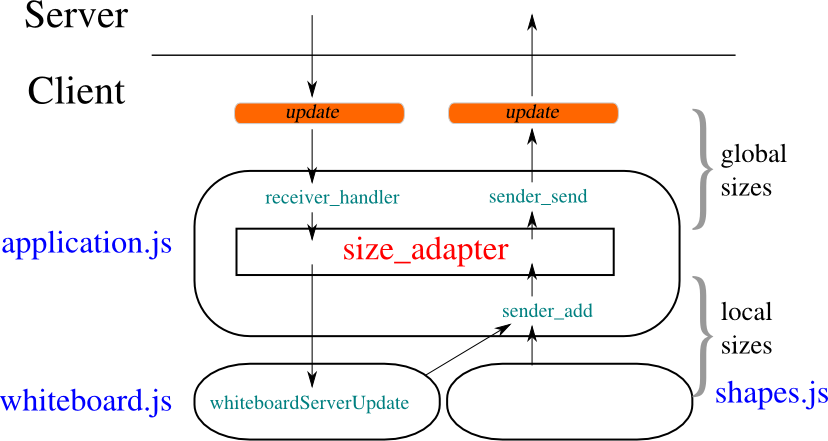
\includegraphics{images/size_adapter.png}

A translation between global units and pixels is performed also on the
server-side, when exporting the whiteboard content to a pdf or image
file.


%___________________________________________________________________________

\hypertarget{security-measures}{}
\section{Security measures}
\label{security-measures}

Some weak security measures were taken, just to discourage users to
try to stole the identity of others, but the taken measures present
several limits so they are intended to provide a reduced level of
security, suitable for an informal use environment, where the trust
isn't a problem, and where the possible damage done by an attacker is
reduced.


%___________________________________________________________________________

\hypertarget{request-signature}{}
\subsection{Request signature}
\label{request-signature}

The main security measure is to not send the plain text form of the
user password with each request, but instead to \emph{sign} each request
with the user password on the client side, so that the server can use
his stored password to verify the signature.

This is accomplished by the \texttt{g{[}'signer'{]}} object on the client side,
and by the \texttt{verify{\_}credentials} function on the server side. This
kind of signature get done just for those modes which require an
authentication, which are defined into the \texttt{{\$}known{\_}modes}
array. Both the \texttt{{\$}known{\_}modes} array and the use of
\texttt{verify{\_}credentials} function can be found into the \texttt{main.php}
file.

The only moment when the password get transmitted in plain text form
through the http channel is when the user registers himself,
associating that password with his name.


%___________________________________________________________________________

\hypertarget{reply-attack}{}
\subsection{Reply attack}
\label{reply-attack}

This kind of security mechanism is prone to a reply attack, because
the signed part of the request is the same for different requests. To
reduce this problem, there is a continuous exchange, between the
server and the client, of a time-dependent value, which makes requests
not reusable after a given time interval.

This time-dependent value is a timestamp, generated and signed by the
server (function \texttt{update{\_}salt} into \texttt{updates.php}), which becomes
part of the data signed from the client (function \texttt{get{\_}signature}
within the \texttt{g{[}'signer'{]}} object into \texttt{common.js}), and then is
checked by the server for each authenticated request. The
\texttt{g{[}'signer'{]}} object has the responsability of keeping the server
timestamp (also called \emph{server salt}) updated, using an ajax channel.

The variable ruling the timestamp validity is
\texttt{{\$}server{\_}timestamp{\_}validity} into \texttt{verify{\_}credentials} into
\texttt{updates.php}, the variable ruling the interval used by the client
for updating the timestamp is \texttt{cycle{\_}timeout} into the
\texttt{g{[}'signer'{]}} object into \texttt{common.js}. If this parameters shall
become configuration variables, the client \texttt{cycle{\_}timeout} value
should be sent from the server to the client (see \href{\#global-variables-directly-sent-from-the-server-to-the-client}{\ref*{global-variables-directly-sent-from-the-server-to-the-client}}).


%___________________________________________________________________________

\hypertarget{timeout-effects}{}
\section{Timeout effects}
\label{timeout-effects}

A timeout is a problem that must be handled at both ends of the
communication, the server and the client. Indeed, the natural handling
for a timeout is a retry, and when retries are in play a protocol
problem arises, to avoid message duplication.

Actually, considering the operations handled through asynchronous
(ajax) requests, it can be seen that many of them don't have
server-side effect, so their duplication is not important. These are
the requests sent with modes: \texttt{read} (\texttt{g{[}'receiver'{]}} object),
\texttt{update{\_}salt} (\texttt{g{[}'signer'{]}} object), \texttt{checkuser}
(\texttt{g{[}'login'{]}} object).


%___________________________________________________________________________

\hypertarget{sender-requests-and-the-send-id}{}
\subsection{Sender requests and the \texttt{send{\_}id}}
\label{sender-requests-and-the-send-id}

The \textbf{only problem} comes with a request sent by the \texttt{g{[}'sender'{]}}
object with the \texttt{write} parameter: this is a request carrying an
\textbf{update}, and repeting it is not safe, so the server must detect and
nullify a duplicated request.

To made the update requests detectable, it is necessary to assign an
identifier to each of them. A new unique identifier must be created on
the client side and verified on the server side, so the two sides must
be synchronized from the client side initialization and through all
request attempts.

This application doesn't mantains a (server side) session state, but
just a whiteboard and an user state, so the \emph{current update
identifier} must be an user variable, sent with the other variables as
seen into \href{\#global-variables-directly-sent-from-the-server-to-the-client}{\ref*{global-variables-directly-sent-from-the-server-to-the-client}}.

The identifier is a variable called \texttt{send{\_}id}. Its value is sent as
a query field with each \texttt{write} request, and incremented separately
by the client and the server in case of success.


%___________________________________________________________________________

\hypertarget{parametric-layout}{}
\section{Parametric layout}
\label{parametric-layout}

Just a short mention about the layout configuration variables. Through
all the code, I tried to refer to those variables as much as possible,
but the layout is not fully parametric currently, and it would be
difficult event to simply state what kind of layout feature should be
modified by the administrator and how. However I always try to refer
to global variables (on the server side) and to server variables (on
the client side) in order to have, at least, a good level of internal
coherence when referring to the same values.


%___________________________________________________________________________

\hypertarget{data-structures}{}
\chapter{Data structures}
\label{data-structures}

This section is very important for the developer, due to the lack of
incapsulation that can affect some data structures. It is important to
mantain a centralized reference for data structures, to preserve their
coherence while they get accessed by several peripheral functions
both in the client and the server side.


%___________________________________________________________________________

\hypertarget{stored-data}{}
\section{Stored data}
\label{stored-data}

Stored data are those which get wrote on the disk by the server side
code, into the files choosen through the configurable variables into
\texttt{configuration.php}.

When the server configuration variable \texttt{{\$}debug} is set to \texttt{true},
for each file read by the server (function \texttt{file{\_}get}) a readable
copy of the content is written on the disk, with the suffix
``-debug''. This can help in fixing issues and for a better
understanding of data structures.

The stored data reside into the \texttt{data/} folder, even if all position
can be configured. This image shows the default structure of the data
folder (lock files are not shown, see \href{\#server-side-concurrency}{\ref*{server-side-concurrency}} for
details on locking):

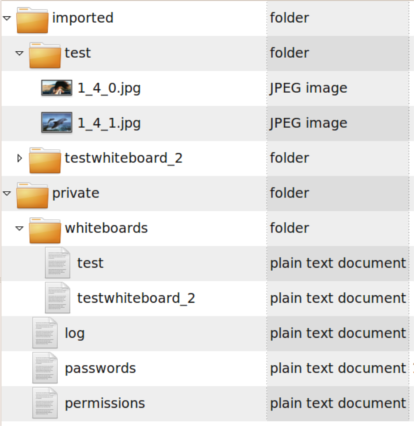
\includegraphics{images/default_structure_data_folder.png}

In the image you can see the folders \texttt{imported} and \texttt{whiteboards},
which get filled and emptied by the server with the creation and
deletion of new whiteboards. For each whiteboard, a file is created
into \texttt{private/whiteboards}, and a folder into \texttt{imported}.

The files \textbf{permissions} and \textbf{passwords} are essential for the
application's operation, so if they are missing they get created
automatically and filled by the server side code with default
content. For this reason, the files aren't present into the
application's distribution (see \href{\#permission-file}{\ref*{permission-file}} for some
details). Also the \texttt{log} file is created by the first server log
message.

As you can see, the imported images stay into a public folder, while
all other data should stay into a private one (although folder's names
can't actually say which permissions were given to those folders).

Two types of data get stored on the server, which are very different:
\begin{itemize}
\item {} 
textual data, usually an encoded form of complex php arrays

\item {} 
images

\end{itemize}

the textual data are often a serialized form of php variables, except
in the case of the permission table (\texttt{{\$}permission{\_}file}) which has a
precise format in order to be easily used from the administrator.

The images are those imported from a pdf file for a user \emph{import}
request, or those grabbed by the web after a user \emph{image create}
action. They are deleted by the server when the user requires the
deletion of the corresponding whiteboard object.

Imported images reside in a folder which is specific for each
whiteboard. The folder is created when there is the need to import the
first image (function \texttt{acquire{\_}image} into \texttt{updates.php}), and
deleted with all its content when the whiteboard is deleted by an user
with the right permissions.


%___________________________________________________________________________

\hypertarget{whiteboard-database}{}
\subsection{Whiteboard database}
\label{whiteboard-database}

The whiteboard database is the most important data repository for the
application. It is specific for each whiteboard, so it can be created
and deleted like whiteboards can be. It contains mainly:
\begin{itemize}
\item {} 
few variables which are global for the whiteboard (mainly counters)

\item {} 
the update database, presented in the initial section \href{\#main-principle}{\ref*{main-principle}}

\item {} 
user data relative to the whiteboard, like size customizations

\end{itemize}

The database is a serialization of a php array whose structure (with
the correct key names) is the following:
\begin{itemize}
\item {} 
database
\begin{itemize}
\item {} 
\texttt{next{\_}upd{\_}id}: identifier for the next update that will be stored

\item {} 
\texttt{next{\_}usr{\_}id}: identifier for the next user that will join this whiteboard

\item {} 
\texttt{delete{\_}count}: the number of objects deleted since the last cleanup

\item {} 
\texttt{updates}\footnotemark[7]: the update database; each update contains the
following fields (those with the star * symbol are added by the
server):
\begin{quote}
\begin{itemize}
\item {} 
\texttt{update{\_}id} *: it is the key of the update in the database array

\item {} 
\texttt{time} *: timestamp when the server added the update

\item {} 
\texttt{madeby} *: user \emph{name} (not user id) of the user from whom the
update came

\item {} 
\texttt{page}

\item {} 
\texttt{objid}: see \href{\#object-id}{\ref*{object-id}} under \href{\#joined-arrays}{\ref*{joined-arrays}}

\item {} 
\texttt{action}

\item {} 
\texttt{parameters}: see \href{\#action-parameters}{\ref*{action-parameters}} under \href{\#joined-arrays}{\ref*{joined-arrays}}

\end{itemize}
\end{quote}

\item {} 
\texttt{uids}: the array of user data pertaining a whiteboard, which is
indexed with each user's id
\begin{quote}
\begin{itemize}
\item {} 
\texttt{username}: a string with the name of this user. This is
unique like the user id, because it is the value the user fills
in to identify himself at the login page.

\item {} 
\texttt{session{\_}id}: a counter which is incremented each time the
application page is sent to the user. This will be used to
build unique object ids on the client side.

\item {} 
\texttt{client{\_}id}: the client identifier, a variable sent by the
client to the server (see \href{\#the-client-identifier}{\ref*{the-client-identifier}} for
details). It is not strictly necessary to store this value, it
could be easily built each time it is needed (function
\texttt{get{\_}user{\_}variables} and function \texttt{login} into
\texttt{updates.php}).

\item {} 
\texttt{slides}: the addres that the user has loaded into the iframe
panel

\item {} 
\texttt{send{\_}id}: a sequence number for client \texttt{write} requests
(see \href{\#sender-requests-and-the-send-id}{\ref*{sender-requests-and-the-send-id}})

\end{itemize}

The following parameters are the layout parameters which a user
can personalize, and which must be kept server side because they
affect the sizes of the root svg element which can't be modifyed
client side. The parameters are set to default values when a new
user is created (function register into updates.php).
\begin{itemize}
\item {} 
\texttt{width}: total width of the whiteboard

\item {} 
\texttt{height}: total height of the whiteboard

\item {} 
\texttt{side{\_}w}: width of the right side pane containing the chat
and the iframe

\end{itemize}
\end{quote}

\end{itemize}

\end{itemize}


%___________________________________________________________________________

\hypertarget{serialize-and-json-encode}{}
\subsubsection{serialize and json{\_}encode}
\label{serialize-and-json-encode}

During the development, I switched from the use of \texttt{serialize} to
the use of \texttt{json{\_}encode} to store the php variables on the disk. I
did this because I found that even the simplest arrays were encoded by
\texttt{serialize} including their indexes, like into the example below:
\begin{quote}\begin{verbatim}
'updates' =>
array (
  1 =>
  array (
    '0'=>1,
    '1'=>1287411219,
    '2'=>'fra',
    '3'=>'0',
    '4'=>'1_4_1',
    '5'=>'image',
    '6'=>'...'
  ),
  2 =>
  array (
    '0'=>2,
    '1'=>1287411224,
    '2'=>'fra',
    '3'=>'0',
    '4'=>'1_4_1',
    '5'=>'move',
    '6'=>'-21.4|-14.9',
  ),
  3 =>
  array (...
\end{verbatim}
\end{quote}

While the string produced by \texttt{json{\_}encode} is more compact (spaces
and newlines added here for readability):
\begin{quote}\begin{verbatim}
"updates":{
        "1":[1,1288003041,"fra","0","1_1_0","path","..."],
        "2":[2,1288003041,"fra","0","1_1_1","path","..."],
        "3":[...
\end{verbatim}
\end{quote}


%___________________________________________________________________________

\hypertarget{permission-file}{}
\subsection{Permission file}
\label{permission-file}

This file is necessary for the application to run, because it rules
the behavior of the application when it comes to give to any user the
permission to do fundamental actions, that are creating, accessing or
deleting any whiteboard.

The file is conceived to be manually edited by the application's
administrator, so it is structured as a ``delimited separed values''
file, with a single space as delimiter. The form of each row must be
the following:
\begin{quote}\begin{verbatim}
<user> <whiteboard> <permissions>
\end{verbatim}
\end{quote}

Where \texttt{<user>} and \texttt{<whiteboard>} can be two regexp, and
\texttt{<permissions>} is a string composed by the letters \texttt{a}, \texttt{c},
\texttt{d}, each one giving, when present, the permission to access, create
or delete, to the given user regexp on the given whiteboard regexp.

This file is missing into the application package, so the
administrator can write one by himself. If he doesn't, the server side
code will create a file with the default rule of allowing everything
to everyone (see function \texttt{check{\_}permissions} into
\texttt{file{\_}access.php}), that is a rule like this:
\begin{quote}\begin{verbatim}
.* .* abc
\end{verbatim}
\end{quote}

This file is just read by the short function \texttt{check{\_}permissions}
into \texttt{file{\_}access.php}, so check out that function to retrieve
detailed informations, as the use of the library functions \texttt{fgetcsv}
to read the file and \texttt{ereg} to evaluate the regular expression.


%___________________________________________________________________________

\hypertarget{password-file}{}
\subsection{Password file}
\label{password-file}

The passwords file is read and written with the same functions used
for the whiteboard databases, in order to store a php variable into
it. The structure of this variable is very simple:
\begin{quote}\begin{verbatim}
array('server_pass' => 'password_s',
      'user_pass'   => array('username1' => 'password_1',
                             'username2' => 'password_2',
                             'username3' => 'password_3');
\end{verbatim}
\end{quote}

The passwords are written when each user registers himself (that is
also the only moment when they go through the http channel in plain
text form).

The \texttt{server{\_}pass} is generated and used by the server to sign the
salt.


%___________________________________________________________________________

\hypertarget{joined-arrays}{}
\section{Joined arrays}
\label{joined-arrays}

The whiteboard makes wide use of joined arrays to handle complex data
structures. This means that an array is translated into a string (with
one-character separators between his elements) at one side of the
transmission, and this string can be split again at the other end,
where the details of the data structure must be read or changed.

For example, this diagram shows how the parameters and other data
pertaining a new action get sent to the server, packed with the use
of \texttt{|}, \texttt{:}, \texttt{;} separators.

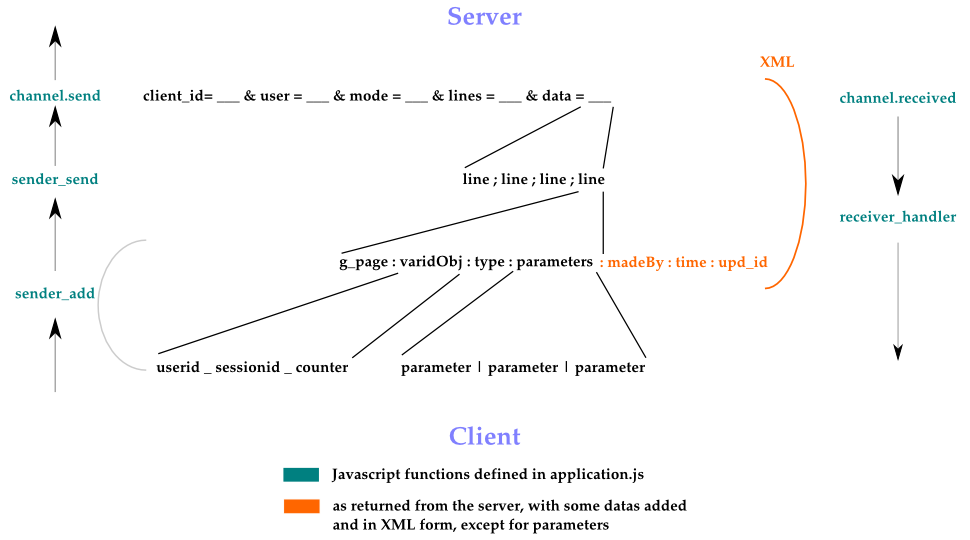
\includegraphics{images/sending_update_separators.png}

Data are encoded on different levels to allow the expansion of certain
fields; for example, the object id structure could (and did) change
over time, and the update parameters change with the different action
type.

The text inserted by the user (for example, into a \texttt{chat} action
update) is escaped (using \emph{urlencoding}) to prevent its content from
interfering with the separators.


%___________________________________________________________________________

\hypertarget{object-id}{}
\subsection{Object id}
\label{object-id}

Each object Id must be unique value into a whiteboard database; it has
the following structure:
\begin{quote}\begin{verbatim}
<user id> _ <session id> _ <object counter>
\end{verbatim}
\end{quote}

like as ``3{\_}35{\_}12''
\begin{description}
\item[{user id}] \leavevmode 
The user id (they start from 1, the value 0 can be used by the
server if it needs to build objects not associating them to any
user).

\item[{session id}] \leavevmode 
The session id is incremented each time a user receives the
application page, and transmitted to the client where it remains
as a global variable. This is the main value that grants the
unicity of the object ids because it is different for each
initialization of the javascript environment (for a given user on
a given whiteboard).

\item[{object counter}] \leavevmode 
It starts from zero when the javascript is initialized, that is
with each new session id.

\end{description}


%___________________________________________________________________________

\hypertarget{server-object-id}{}
\subsubsection{Server object id}
\label{server-object-id}

The server doesn't have an user or session id, however there is a case
where it has to build objects with an unique object id. This happens
into the function \texttt{import} (file \texttt{updates.php}), where several pdf
pages are turned into images and inserted into the whiteboard.

The object id used this time has the form:
\begin{quote}\begin{verbatim}
<user id> _imported_ <page counter>
\end{verbatim}
\end{quote}

And it is unique anyway, because when the import operation is
performed, each page that will be fill with a pdf page is cleared
before, so two objects named \texttt{{\_}imported{\_}} with the same page counter
can't exist (the \texttt{<user id>} is thus not strictly necessary).


%___________________________________________________________________________

\hypertarget{action-parameters}{}
\subsection{Action parameters}
\label{action-parameters}

The handling of action parameters is quite unconfortable for the
developer: here I will describe the current state of the code, while
in the next session I will discuss drawbacks and alternatives to the
use of joined arrays to encode this data.

The parameters can change depending on the type of action, and must be
accessed in a coherent way through all the code. The actual order of
parameters for an action is decided when the update string is created,
that is on the client side, in all the places before the
\texttt{sender{\_}add} function is called.


%___________________________________________________________________________

\hypertarget{shape-action}{}
\subsubsection{Shape action}
\label{shape-action}

Each shape defines its list of parameters, wich it will use to read
updates to the server, to send them, and sometimes to clone an
existent shape for editing. Here is a snippet of a shape defining its
attributes (taken from the file \texttt{shapes.js}):
\begin{quote}\begin{verbatim}
function line(){
    var att = ['opacity','stroke-width','x1','y1','x2','y2'];
\end{verbatim}
\end{quote}

These definitions must be taken as the reference for the meaning of
parameters for shape actions (line, path, rect, circle, polygon,
polyline, etcetera), but remember that the actual index must be
incremented by two, because each shape has two default attributes
defined into the parent class \texttt{shape}, as can be seen into this
snippet taken by that class:
\begin{quote}\begin{verbatim}
// The colors are common attributes between all shapes
var colors = ['stroke', 'fill'];
object.att = colors.concat(att);
\end{verbatim}
\end{quote}

For example, the final positions of parameters in a \texttt{line} action
will be:
\begin{quote}\begin{verbatim}
stroke | fill | opacity | stroke-width | x1 | y1 | x2 | y2
0        1      2         3              4    5    6    7
\end{verbatim}
\end{quote}


%___________________________________________________________________________

\hypertarget{other-actions}{}
\subsubsection{Other actions}
\label{other-actions}

I will summarize in a table the parameters for all actions which are
not shapes (line, circle, rect, path, etcetera are excluded). For each
action, I include the file from where the corresponding \texttt{sender{\_}add}
function is called (this can be easy wiewed using \texttt{grep sender{\_}add
*.js}). Actions \texttt{clear} and \texttt{delete} don't have parameters.

\leavevmode
\begin{longtable}[c]{|p{0.315\locallinewidth}|p{0.315\locallinewidth}|p{0.315\locallinewidth}|}
\caption{Parameters for not-shape actions}\\
\hline
\textbf{
Action
} & \textbf{
Parameters
} & \textbf{
File
} \\
\hline
\endhead

move
 & 
translation{\_}x {\textbar} translation{\_}y
 & 
whiteboard.js
 \\
\hline

chat
 & 
escaped{\_}text
 & 
chat.js
 \\
\hline

slides
 & 
escaped{\_}url
 & 
menu.js
 \\
\hline

clear
 & 
\emph{clear}
 & 
whiteboard.js
 \\
\hline

delete
 & 
\emph{delete}
 & 
whiteboard.js
 \\
\hline
\end{longtable}

You can see that the files roughly correspond to the position of the
user interface element that the user activates to perform a given
action.

For actions without parameters, usually a copy of the action type (for
example \texttt{delete} for the \emph{delete} action) is used as parameter, to
avoid problems found while parsing empty XML fields with Internet
Explorer (there is a comment on this into the main \texttt{for} cycle into
\texttt{receiver{\_}handler} into application.js). The copy of the action type
is filled automatically by \texttt{sender{\_}add} when the \texttt{parameter}
argument is missing or it is an empty array.


%___________________________________________________________________________

\hypertarget{drawbacks-and-alternatives-to-the-use-of-joined-arrays}{}
\subsection{Drawbacks and alternatives to the use of joined arrays}
\label{drawbacks-and-alternatives-to-the-use-of-joined-arrays}

The use of joined arrays has several advantages, like easiness of
implementation and an efficient use of storage space, but it also
presents severe drawbacks when considering readability and
maintainability of the code, since the developer has to use positional
parameters in a coherent way each time he tries to parse the format.


%___________________________________________________________________________

\hypertarget{joined-arrays-for-the-update-structure}{}
\subsubsection{Joined arrays for the update structure}
\label{joined-arrays-for-the-update-structure}

The handling of this joined array has been eased introducing a
variable which associates labels to positional indexes. This is the
global variable \texttt{{\$}u{\_}keys}, defined at the top of \texttt{updates.php} and
used just within this file. This variable is used to grant the
coherence of functions which access the update on the server side (all
these functions stay into \texttt{updates.php}), while the database remains
free of redundant labels; however, the syntax can sometimes turn messy
like in this example (taken from function \texttt{cleanup}):
\begin{quote}\begin{verbatim}
...
// Second pass: remove cleared or deleted objects
foreach ($updates as $upd_id => $update){
    $page  = $update[$u_keys['page']];
    $objid = $update[$u_keys['objid']];
    $remove = false;
    if (isset($clear_collection[$page])){
        if ($clear_collection[$page] > $upd_id)
            $remove = true;
    }
    else if (isset($delete_collection[$objid])){
        // Check if we have to remove the image from the filesystem
        if($update[$u_keys['action']] == 'image')
            delete_image($update[$u_keys['parameters']], $wb);
        $remove = true;
    }
    if ($remove)
        unset($updates[$upd_id]);
}
...
\end{verbatim}
\end{quote}

There is another coupling between the client and the server related to
the order of update fields: it occurs when an update is first sent
from the client to the server. It is the programmer, this time, that
must ensure the coherence between the client side function
\texttt{sender{\_}add} into \texttt{application.js} and the server side function
\texttt{write} into \texttt{updates.php}. These functions are at the two end
points of the transmission of a new update. This coupling could be
eliminated using JSON as data format for update upload.

With regard to the last transmission of the update from the server
back to the client, XML is used due to the ajax technology, so some
textual labels must be given into \texttt{read}, which will be transmitted
to the client together with the data in XML form; so there are no
problems with the positional parameters in this case. The encoding and
parsing for update download could probably be simplified using JSON as
data format.


%___________________________________________________________________________

\hypertarget{joined-arrays-for-the-action-parameters}{}
\subsubsection{Joined arrays for the action parameters}
\label{joined-arrays-for-the-action-parameters}

The use of positional parameters is quite a problem with the action
parameters handling, because action parameters get accessed by
different parts of both server and client side code, and the developer
has to check manually if each index is the right one.

The parts of the code that are depending on the parameter positions
range from the shape (and chat message) creation functions on the
client side, to the server side functions which export the whiteboard
contents in different formats, to other server side functions (for
example, the acquisition on the server of a newly inserted image).

The alternative would be to have textual labels associated to each
field, this would be much readable and much maintainable, but this
would come at a cost: how to store these labels when the actions get
written into the database?

It is clear that all actions of a given type stored into the database
should have the same format, so there's no reason to repeat the
format; a centralized reference should exist to hold the appropriate
labels.

This \emph{label reference} would be an array with the form:
\begin{quote}\begin{verbatim}
line:    'stroke', 'fill', 'opacity', 'stroke-width', ...
polygon: 'stroke', 'fill', 'fill-opacity', ...
\end{verbatim}
\end{quote}

This label reference should be either transmitted between the client
and the server, or defined two times, once on the client and once on
the server side. I think the latter is the best solution, but the two
structures should be syntactically as similar as possible, to be
easily compared and updated by the developer in case of change

As already seen, on the client side, each shape defines its parameters
(in the file \texttt{shapes.js}). This comes from the object oriented
paradigm, in an effort to make each shape opaque and independent from
the rest of the code.

Wheter is better or not to define shape parameters within each shape,
I think it is a subjective matter; however, a centralized \emph{label
reference} could be added to the server side, and this would probably
be a maintainability improvement.

Until now I have done without a label reference, but I find that the
necessity could come in the future to use textual labels instead of
numerical parameters in the server side, that's why I included this
short analysis into the documentation to explain how to add it.


%___________________________________________________________________________

\hypertarget{specific-solutions-and-workarounds}{}
\chapter{Specific solutions and workarounds}
\label{specific-solutions-and-workarounds}

In this section I collect several solutions that don't came from the
project of the application, but just from the efforts of implementing
such project. If an issue is spotted and fixed and his solution is
worth writing, or if a workaround is used to avoid a specific problem,
this is the place where to write it.


%___________________________________________________________________________

\hypertarget{use-of-svgweb}{}
\section{Use of svgweb}
\label{use-of-svgweb}

These are some techniques used into the client side (whiteboard.js),
to allow svgweb to do is work, translating svg functions and objects
to flash ones. Some of these recommendations can also be found on
svgweb official documentation.


%___________________________________________________________________________

\hypertarget{generic-notes}{}
\subsection{Generic notes}
\label{generic-notes}

The variable svgns is provided by the library, containing the svg
namespace.

On the ``svg'' node, width and height must be specified as svg
attributes, not into the svg style attribute.

Dom method ``getElementsByTagname'' must be replaced with
``getElementsByTagNameNS(g{\_}svgNS, '' and ``createElement('' with
``createElementNS(g{\_}svgNS, ''

Instead of using '.setAttribute' for event listening, and instead of
using html ``handler'' attribute, use '.addEventListener' for event
listening.

Svgweb requires a boolean in svg createTextNode invocation (a 'true'
as last argument), but this boolean must be omitted if the script is
writing a regular html text node outside the svg.

Svgweb (``gelatinous cube'' version, at least) \textbf{doesn't support the
``stopPropagation'' method}.

To update the text, element.textContent=``new text'' doesn't works; it
is necessary to create a new text node with document.createTextNode,
to delete the previous content with element.removeChild, and to append
the new node with element.appendChild.

Text nodes don't inherit event listeners from the ``svg'' root node, so
we need to add the handlers to a text node when it is created into
'createGroup'. Doing this way however svgweb forwards the 'mousedown'
event to the text node but also to the ``svg'' node behind, so I added a
check in ``handleMouseDown'' that nullifies the second call made by the
``svg'' node (this can be related to issue 497 that was fixed into the
latest svgweb release, owlefant, so I'm not sure this problem still
stands).


%___________________________________________________________________________

\hypertarget{image-and-anchor-support}{}
\subsection{Image and anchor support}
\label{image-and-anchor-support}

Google chrome shows images only outside a text element, and shows
anchors ('a' tags) only inside a text element but not into a tspan
element. This is the reason why there are tree different buttons:
text, link, image, which correspond to a different structure of the
included SVG elements.

The following list is a set of reasons why links have been implemented
like text nodes, with an hidden empty {\textless}tspan{\textgreater} inside to identify them,
and they are opened with javascript window.open()
\begin{itemize}
\item {} 
Anchors can't be correctly moved with flash: when trying to move
them the browser navigates them, so it must be avoided their default
handler (but preventDefault at the beginning of handleMouseDown
seems not to be enough, and stopPropagation is not supported by
svgweb).

\item {} 
Anchors appear black with flash renderer (it doesn't honor style
attribute).

\item {} 
With the firefox native renderer, links get opened in a new window,
while with flash they get opened into the same window

\end{itemize}

Image attributes are set together with the setting the xlink
attribute. While I was trying to reorganize the code I kept these
assignments always near, because it seemed to be the only way to make
flash actually show the images. Maybe with the new versions of svgweb
this won't be a problem, but I write this remainder to help in case of
weird problems.


%___________________________________________________________________________

\hypertarget{resize-the-svg-root-node}{}
\subsection{Resize the SVG root node}
\label{resize-the-svg-root-node}

Currently, all user interfaces which resize the SVG canvas require a
refresh of the whole page: this came from the impossibility to
dinamically resize the SVG root element (the \texttt{<svg>} tag), and I
will summarize briefly the attempts made in this direction.

Dynamically change the sizes of the svg root works fine with
firefox/native, but doesn't works with the flash renderer, as it
confirmed also by the issue 427 (see the svgweb issues), at list at
the date of November the 3dh, 2010.

I tried a different way, deleting and rebuilding the svg root node,
but there were errors with sizes (the height was always wrong) and
some contents of the root node were not showed properly. Svgweb
doesn't even allowed to copy the content of the root node on a
temporary variable to append them to a new root node, and so a
\texttt{refresh} request to the server was needed in any case.

From the test made I considered the library support for this kind of
features as unstable, and to speed up the development I decided to use
the simplest method, refreshing the whole page with a new request to
the server. This came also from the consideration that the resize
action is quite infrequent.


%___________________________________________________________________________

\hypertarget{coordinates-within-the-svg-canvas}{}
\section{Coordinates within the svg canvas}
\label{coordinates-within-the-svg-canvas}

This section mainly describes the kind of work done by the function
\texttt{skew} defined into \texttt{whiteboard.js}, to adapt coordinates into the
svg environment. Many of the outcomings written here derived from
direct testing.

Types of coordinates on which to apply an offset:
\begin{itemize}
\item {} 
coordinates from mouse events (target.clientX and target.clientY)

\item {} 
coordinates from nodes position (target.getAttribute)

\end{itemize}

Browser to consider when applying offsets:
\begin{itemize}
\item {} 
firefox/native

\item {} 
chrome/native

\item {} 
flash renderer (mainly on explorer)

\end{itemize}

Effects that modify the position:
\begin{itemize}
\item {} 
the origin of the svg root node

\item {} 
the scrolling state of the page

\end{itemize}

Operations involved:
\begin{itemize}
\item {} 
object creation (pure mouse coordinate)

\item {} \begin{description}
\item[{object moving (coordinates from position plus difference between}] \leavevmode 
mouse coordinates)

\end{description}

\item {} 
object editing: edited point (pure mouse coordinate)

\item {} 
object editing: other points (coordinates from original nodes positions)

\end{itemize}


%___________________________________________________________________________

\hypertarget{browser-behavior-for-svg-offset}{}
\subsection{Browser behavior for svg offset}
\label{browser-behavior-for-svg-offset}
\begin{description}
\item[{Firefox (native renderer) (3.5.9):}] \leavevmode 
Mouse coordinates (retrieved with target.clientX and target.clientY)
are absolute, so we must subtract the position of the svg root,
before assigning those values to attributes of svg nodes. Also other
target.getAttribute (used into init{\_}start) values are absolute.

\item[{Chrome (native):}] \leavevmode 
Mouse coordinates (target.clientX and clientY) are absolute like in
firefox/native, but nodes coordinates (target.getAttribute) are
relative to the svg root and shouldn't be changed. For this reasons,
the function ``skew'' needs to know if it is adapting a node
coordinate or a pointer coordinate (boolean parameter ``pointer'').

\item[{Flash renderer (tested on firefox):}] \leavevmode 
Mouse coordinates (target.clientX) and target.getAttribute are
relative to the svg root, so no further change has to be made.

\end{description}


%___________________________________________________________________________

\hypertarget{browser-behavior-for-scroll-state}{}
\subsection{Browser behavior for scroll state}
\label{browser-behavior-for-scroll-state}
\begin{description}
\item[{Explorer(6)/flash:}] \leavevmode 
Page scroll state is written into document.body.scrollLeft or
.scrollTop. This must be applied to every type of coordinates.

\item[{Firefox/native:}] \leavevmode 
Page scroll state is written into window.pageXOffset or
.pageYOffset. This must be applied to every type of coordinates.

\item[{Chrome/native:}] \leavevmode 
Just apply scroll skew to pointer coordinates

\item[{Firefox/flash:}] \leavevmode 
Doesn't need any skew due to the scrolling state

\end{description}


%___________________________________________________________________________

\hypertarget{testing-environment-and-methods}{}
\chapter{Testing environment and methods}
\label{testing-environment-and-methods}


%___________________________________________________________________________

\hypertarget{browsers}{}
\section{Browsers}
\label{browsers}

The test is quite a problem in a project like this, with several kind
of execution environments. The amount of possible execution conditions
is made up by the number of different browsers, but also by the
renderer in use (about two choiches for each browser, the native
renderer and the flash one), and by the different versions of the
flash renderer.

The used method has been to choose a main browser for initial tests,
and then try other browsers with a lower frequence. The browser used
mainly was firefox (3.5) with its native renderer, due to the advantage
provided by the ``firebug'' plugin (but also google Chrome offers some
developement tools with the same functionalities).

The second browser for test frequency has been Internet Explorer with
the flash renderer. While firefox has quite a stable support to web
standards through its versions, the support provided by Internet
Explorer can change strongly between different versions (many features
can be missing on older versions), so I used an old version (6) in the
purpose of having good code portability.

The third browser was google chrome, with its native renderer. It
behaved mostly like firefox, but the renderer showed some differences
in the handling of svg (pointer coordinates inside the svg canvas,
syntax for polygons/polylines).

These browsers have been used for the tests during the developement,
while I left Opera, Safari, and Explorer 7 and 8 just for a final
test.


%___________________________________________________________________________

\hypertarget{debugging-javascript-in-explorer}{}
\section{Debugging Javascript in Explorer}
\label{debugging-javascript-in-explorer}

The debug difficulties with Explorer often imposed to proceed by
little steps. Javascript errors are showed generically in Explorer,
with a line number that doesn't corresponds to any file (and the
javascript file from which the error comes is not showed).

Since the adoption of the ``microsoft script debugger'', the spot of
javascript errors on Explorer has speeded up a lot, but with complex
object structures (and function literals), the debugger can still lose
its usefulness, becoming unable to locate and show the correct error
line. A very cautious approach to the developement of new client side
functions must therefore still be used.

Given that many javascript errors occurred only on explorer (for the
implementation differences, and because this is the environment where
svgweb comes in play), the debug process for such errors became
occasionally very slow and imposed a tight test cycle when developing
new client side features.

A bigger problem comes with the use of the flash renderer with svgweb,
when a behavior is different from that of the native
renderer. Usually, the first step I did when I found problems was to
set the \texttt{svg.render.forceflash} flag to \texttt{true}, to use the flash
renderer also with firefox (this flag is set through a \texttt{meta}
included before the \texttt{svg.js} script, see the function
\texttt{common{\_}frame} into \texttt{markup{\_}send.php}).

Using firefox, even if the actionscript objects are not accessible, it
is possible to use the methods provided by svgweb through the
javascript console, and to follow the javascript execution flow (and
variable changes) in details. The flash renderer run under firefox
behaved \emph{almost} always like the one run under explorer.


%___________________________________________________________________________

\hypertarget{hardware}{}
\section{Hardware}
\label{hardware}

The machine upon which all test have been made has the following
characteristics:
\begin{itemize}
\item {} 
processor: Intel Pentium M 1.70 Ghz

\item {} 
memory: 1 GB

\end{itemize}

Which where (obviously) widely sufficient to run the client side code,
even with several open browsers or with explorer running into a
virtual machine.


%___________________________________________________________________________

\hypertarget{performance-problems}{}
\subsection{Performance problems}
\label{performance-problems}

One performance problem concerned explorer, inside the virtual
machine, that randomly showed an excessive slowness while showing the
page served by apache on localhost; in this cases, a restart of
explorer fixed the problem.

The server reaches performance limits when handling with graphic
functions (import and export), that indeed work in an asynchronous
manner with respect to user activity on the whiteboard. Especially,
the import of a long (many pages) pdf file into the whiteboard may
take some time and requires full processing power and a substantial
amount of memory (200MB of memory needed to convert a 715KB pdf file
to 27 jpeg images whose cumulating size was 1.7MB).


%___________________________________________________________________________

\hypertarget{directions-for-further-development}{}
\chapter{Directions for further development}
\label{directions-for-further-development}


%___________________________________________________________________________

\hypertarget{prepare-for-html5}{}
\section{Prepare for HTML5}
\label{prepare-for-html5}

In an application like this, that makes a wide use of the front-end
web technologies, an innovation like HTML5 can't be ignored and
instead must be looked as an important opportunity to improve the
quality of the application. A deeper analysis is required, but I can
list here a short set of HTML5 features which can impact on this
application.
\begin{itemize}
\item {} 
the local storage can allow to eliminate the \texttt{window.name} hack
for passing state through different pages

\item {} 
the availability of an offline cache could allow users to make their
drawings while disconnected from the server, and keep them safely
until the moment for sharing it comes\footnotemark[8]

\item {} 
the form validation would be eased

\end{itemize}

But the feature that could completely change the application
architecture is the incoming of \textbf{HTML5 websockets}. These would at
least eliminate the trick used for \href{\#emulating-a-client-push-behavior-with-the-http-technology}{\ref*{emulating-a-client-push-behavior-with-the-http-technology}}, but their real potential is the
possibility of a \emph{peer to peer} communication model between the
clients, with the server acting as a coordinator.

Even if this possibility is exciting and may lead to a true revolution
for many web applications, websockets are currently supported just by
the Safari and Chrome web browsers, and are still under strong
development. Even their bare
\href{http://dev.w3.org/html5/websockets/}{specification} is still a
draft.


%___________________________________________________________________________

\hypertarget{the-canvas-element}{}
\subsection{The canvas element}
\label{the-canvas-element}

A mention must be done to the \texttt{<canvas>} element which is going to
be widely supported by the browsers which will support HTML5. The fact
that the application is based upon SVG can look like a wrong choice
from this point of view, but please consider that also SVG will be
supported by the same browsers, so it's not so easy to decide which
technology is better. Several articles on the web debate about the
differences between the two methods, and I think that here is better
to speak about the application structure and how much is it binded to
the SVG standard.

The two files that handle the application drawing functions are
\texttt{whiteboard.js} and \texttt{shapes.js}. The first is influenced by the
SVG standard only for the application of move actions and the use of
SVG groups to handle the objects on the whiteboard.

The second file, \texttt{shapes.js}, is tightly binded to the SVG standard,
given that many operations automatically copy the attributes from the
\emph{update} array to an SVG element, and vice-versa. To change the
structure of \emph{update} strings is possible and it will have
consequences, on the server side, mainly on the export functions.

These considerations could be valid if we wanted to switch from SVG to
another vectorial format, but \textbf{the main problem} is that \textbf{vector
graphics} is the obvious choice for having elements that user \textbf{can
change} over time. It looks to me that the \texttt{<canvas>} element is
thought for drawing and overlay the space with consecutive drawing
actions, but not for the interaction or manipulation of a shared
content. However my knowledge of \texttt{<canvas>} use is rather limited,
and considering that its use and support may evolve with time, this is
an alternative to keep in mind.


%___________________________________________________________________________

\hypertarget{administration-panel}{}
\section{Administration panel}
\label{administration-panel}

Until now, some complex functions (add users, add and delete
whiteboards) have been embedded into the present controls, and some
others (define user permissions) have been moved to a text file to be
manually edited, but an administration panel will be surely needed to
allow a better management of the application.

For example, a function which is currently missing is an easy way to
reset the password of a specific user. The passwords are encoded in
JSON format, and using \texttt{base64{\_}encode} so it's not possible to edit
them by hand.

The current structure of the application uses very few pages so it is
not straightforward to add a new one, however I write here some steps
to follow in order to add this functionality:
\begin{itemize}
\item {} 
\texttt{passwords} or \texttt{configuration.php} should hold the superuser
name

\item {} 
The \texttt{checkuser} server-side function should return a third value
(other than \texttt{used} and \texttt{notused}), \texttt{superuser}.

\item {} 
The login page should show a different button to access to the panel

\item {} 
The contents of the panel should be added, that means:
\begin{itemize}
\item {} 
new modes inside main.php

\item {} 
a new \texttt{markup{\_}send} page

\item {} 
a new javascript file

\end{itemize}

Otherwise the controls for operations limited to the administrator
could appear directly into the login page, but this isn't a coherent
design of the login page.

\end{itemize}

Make sure to check again the superuser identity also on the server
side.


%___________________________________________________________________________

\hypertarget{execution-of-the-whiteboard-as-a-cgi}{}
\section{Execution of the whiteboard as a CGI}
\label{execution-of-the-whiteboard-as-a-cgi}

Initially, the whiteboard was conceived with the idea to execute it
also like a CGI, if needed.

The main solution on this purpose was to parse the query string in two
ways, introducing a function that retrieved the query fields either
from the {\$}{\_}REQUEST php global variable, or from the {\$}{\_}ENV global
variable.

The capability of being executed as a CGI was considered less
important later, and the initial query string parsing was removed from
the code.


%___________________________________________________________________________

\hypertarget{web-resources}{}
\chapter{Web resources}
\label{web-resources}
\begin{description}
\item[{\href{http://help.dottoro.com/index.php}{dottoro web reference}}] \leavevmode 
Contains informations about the support of each browser for each
aspect of css, html, and javascript languages. It is very useful
to avoid spending a lot of time for debug. Unfortunately, it
doesn't covers SVG.

Be warned that, although this reference can be very useful the
most of the times, some attribute may still be missing (for
example I didn't found the innerHTML property as belonging to an
iframe object).

\item[{\href{http://code.google.com/p/svgweb/issues/}{svgweb issue page}}] \leavevmode 
Together with the svgweb mailing list, this is the first place to
search for parts of the SVG standard which are not fully supported
by the library

\end{description}


%___________________________________________________________________________

\hypertarget{notes}{}
\chapter{Notes}
\label{notes}
\footnotetext[1]{
While a complete rewriting of the client code
would probably be convenient, there wasn't a strict need to
perform it, and I was unable to evaluate the benefits of such
an expensive work. So I decided to use the object oriented
paradigm for the newly developed parts, and to convert only the
more complicated and important parts of the existent code, that
means the core whiteboard logic (resulting into the shape
object) and the ajax channel management (resulting into the
channel object).
}
\footnotetext[2]{
The definition of these two steps seems
quite logical and clean, but it presents a performance
weakness: when the login page or the application page is sent
into the \emph{markup send} step, another database access must be
performed. This comes because the login page requires a new
salt, and the application page requires data which must be
specific for each user; the problem is that the database access
was likely already made during the \emph{update} step, by a function
that doesn't cares about the kind of page that will be sent as
output. The \emph{update} functions could be changed in order to
retrieve directly the data also for the output, but I think
that the problem is negligible currently, because the login and
application pages get sent quite seldom to the user, comparing
with other server modes.
}
\footnotetext[3]{
Note that the concurrency hasn't been tested
adequately due to the technical difficulties implied into this
kind of tests. The current solution is based on \textbf{flock}, but
the php manual page for \href{http://www.php.net/manual/en/function.flock.php}{flock} tells about
several limitations, of which the biggest is with multithreaded
server API. However, if flock will result unadeguate to grant
an exclusive lock on the desired files, it will be sufficient
to change the method used by the functions into
\texttt{file{\_}access.php}. The overall architecture will remain
valid.
}
\footnotetext[4]{
Into the function \texttt{file{\_}get} into
\texttt{file{\_}access.php} I use file{\_}get{\_}contents because I had a
problem with fread.  It turned out that filesize({\$}file) wasn't
giving a good value, so junk bytes were read and the parser of
'unserialize' showed errors while reading again the file. The
errors occurred just when the file got opened with the 'r+'
mode, while with the 'r' mode no errors were made on
unserializing.  The problem has been avoided using function
file{\_}get{\_}contents instead of fread.  Maybe the problem was
caused by a wrong use of ftruncate and rewind into
database{\_}put, and is fixed now because file{\_}get{\_}contents does
some kind of parsing. ftruncate fills the file with NULL ASCII
bytes until it reaches the given length, I give length zero,
anyway. All these problems appeared while I was using
\texttt{serialize} to store the data; actually, I use
\texttt{json{\_}encode} instead, because it uses a format which is more
compact.
}
\footnotetext[5]{
Another possibility would be to use SVG relative
(percentual) measure units, but this isn't supported for paths
(maybe there is a workaround manipulating the viewport), and
the overall support of svgweb for this feature must be tested
(at the 22 october 2010 there is just the issue 512 related to
the use of percent units). Even using the percentual units, two
conversions should be done for the mouse input and when
exporting the whiteboard content.
}
\footnotetext[6]{
How much does \emph{almost} means depends from the ratio
between the \texttt{cycle{\_}timeout} value defined into the
\texttt{g{[}'receiver'{]}} object and the overall cycle time, including
the \texttt{server{\_}update{\_}timeout} defined into
\texttt{configuration.php}.
}
\footnotetext[7]{
Currently, the assumption is made that updates are
ordered. This must be considered if a real database is going to
be used in place of the current file. For example into the
server side \texttt{import} function (file \texttt{updates.php}), a page
is cleared (\texttt{clear} update) before a new image (\texttt{image}
update) is inserted in the page. Inverting the order of these
two updates will lead to a result which is completely wrong.
}
\footnotetext[8]{
Actually it should be quite easy to implement. The objects
which implement a channel into the application page
(\texttt{g{[}'receiver'{]}}, \texttt{g{[}'sender'{]}} and \texttt{g{[}'signer'{]}}) should
handle the error condition of an unavailable server asking to
the user if he wants to work in \emph{offline mode}. With a clear
signalation of this condition to the user, It could freely draw
and his updates would be stored into the \emph{sender buffer}. The
application should remember its state, and when the client asks
to look for the server again, the \texttt{g{[}'signer'{]}} object should
be the first to operate, asking for an updated server salt.
}

\end{document}
